 %%%%%%%%%%%%%%%%%%%%%%%%%%%%%%%%%%%%%%%%%%%%%%%%%%%%%%%%%%%%%%%%%%%%%%%%%%%%%%%%
%2345678901234567890123456789012345678901234567890123456789012345678901234567890
%        1         2         3         4         5         6         7         8

\documentclass[letterpaper, 10 pt, conference]{ieeeconf}  % Comment this line out if you need a4paper

%\documentclass[a4paper, 10pt, conference]{ieeeconf}      % Use this line for a4 paper

\IEEEoverridecommandlockouts                              % This command is only needed if 
                                                          % you want to use the \thanks command

\overrideIEEEmargins                                      % Needed to meet printer requirements.

%In case you encounter the following error:
%Error 1010 The PDF file may be corrupt (unable to open PDF file) OR
%Error 1000 An error occurred while parsing a contents stream. Unable to analyze the PDF file.
%This is a known problem with pdfLaTeX conversion filter. The file cannot be opened with acrobat reader
%Please use one of the alternatives below to circumvent this error by uncommenting one or the other
%\pdfobjcompresslevel=0
%\pdfminorversion=4

% See the \addtolength command later in the file to balance the column lengths
% on the last page of the document

% The following packages can be found on http:\\www.ctan.org
\usepackage{graphicx} % for pdf, bitmapped graphics files
%\usepackage{epsfig} % for postscript graphics files
%\usepackage{mathptmx} % assumes new font selection scheme installed
%\usepackage{times} % assumes new font selection scheme installed
\usepackage{amsmath} % assumes amsmath package installed
%\usepackage{amssymb}  % assumes amsmath package installed
\usepackage{url}

\title{\LARGE \bf
COMP 551 Kaggle Competition: Classification of Modified MNIST*
}


\author{Yingnan Zhao$^{1}$, Vincent d'Orsonnens$^{2}$ and Hamed Layeghi$^{3}$% <-this % stops a space
\thanks{*Kaggle Team name: BetaGo, Best Score: 0.95899}% <-this % stops a space
\thanks{$^{1}$Yingnan Zhao, Student ID: 260563769, Electrical Engineering, 
        McGill University,
        {\tt\small nan.zhao2@mail.mcgill.CA}}%
\thanks{$^{2}$Vincent d'Orsonnens, Student ID: 260746099, Software Engineering, McGill University, 
        {\tt\small vincent.dorsonnens@mail.mcgill.ca}}%
\thanks{$^{3}$Hamed Layeghi, Student ID: 260524499, Electrical Engineering, McGill University, 
	{\tt\small hamed.layeghi@mail.mcgill.ca}}%
}

\begin{document}



\maketitle
\thispagestyle{empty}
\pagestyle{empty}


%%%%%%%%%%%%%%%%%%%%%%%%%%%%%%%%%%%%%%%%%%%%%%%%%%%%%%%%%%%%%%%%%%%%%%%%%%%%%%%%
\begin{abstract}
This paper provides the report for the Kaggle Competition (assignment 4) of COMP 551 using the provided Modified MNIST dataset. The dataset includes a set of 8-bit grayscale images that include 2 or 3 digits of different sizes that are rotated and scaled from the classic MNIST dataset. The goal is to design Machine Learning algorithms that identify the biggest digit in each image. Several algorithms have been used in the report. First, the logistic regression and linear SVM are used which lead to relatively lower precisions. Second, a forward neural network completely developed by the team was implemented. Finally, a convoluted neural network was trained and tested on the preprocessed dataset which showed the best performance.  
\end{abstract}


%%%%%%%%%%%%%%%%%%%%%%%%%%%%%%%%%%%%%%%%%%%%%%%%%%%%%%%%%%%%%%%%%%%%%%%%%%%%%%%%
\section{INTRODUCTION}

The MNIST database \cite{MNISTcreators} is a set of handwritten images that is popular for training and testing of Machine Learning algorithms \cite{wiki:MNIST}.

\section{PREPROCESSING}
The provided images in the Modified MNIST include 3 numbers that are rotated and scaled from the MNIST dataset and are written on random backgrounds.
Some samples of the train dataset with their associated outputs are shown in Figure \ref{fig:original}
\begin{figure}[h]
	\begin{center}
		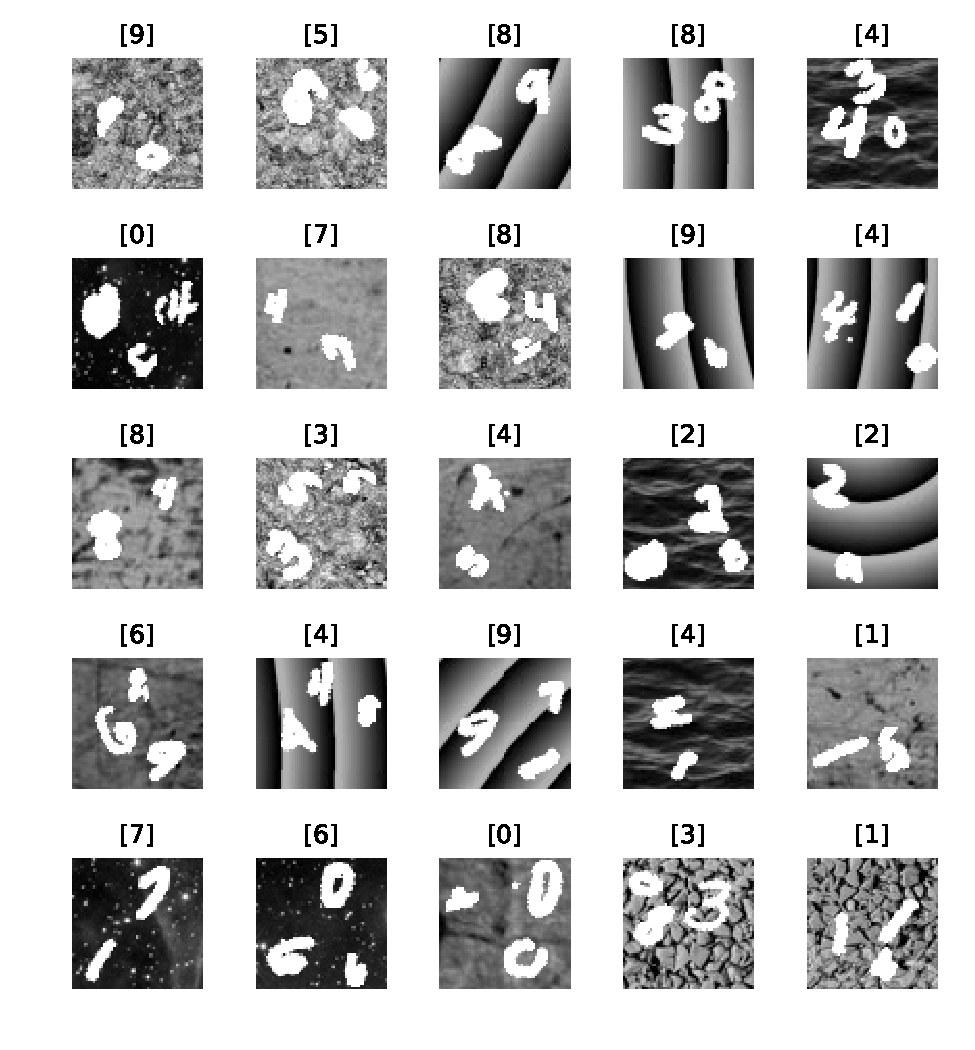
\includegraphics[width=0.4\textwidth]{figures/originalDataset.pdf}  % The printed column width is 8.4 cm.
		\caption{25 Random Samples of the original train dataset}
		\label{fig:original}
	\end{center}
\end{figure}
 The format for the images is 8-bit grayscale image, thus each pixel has 256 shades of gray represented by numbers 0 (black) to 255 (white) as shown in Figure \ref{fig:maxeig2}.

	
\begin{figure}[h]
	\begin{center}
			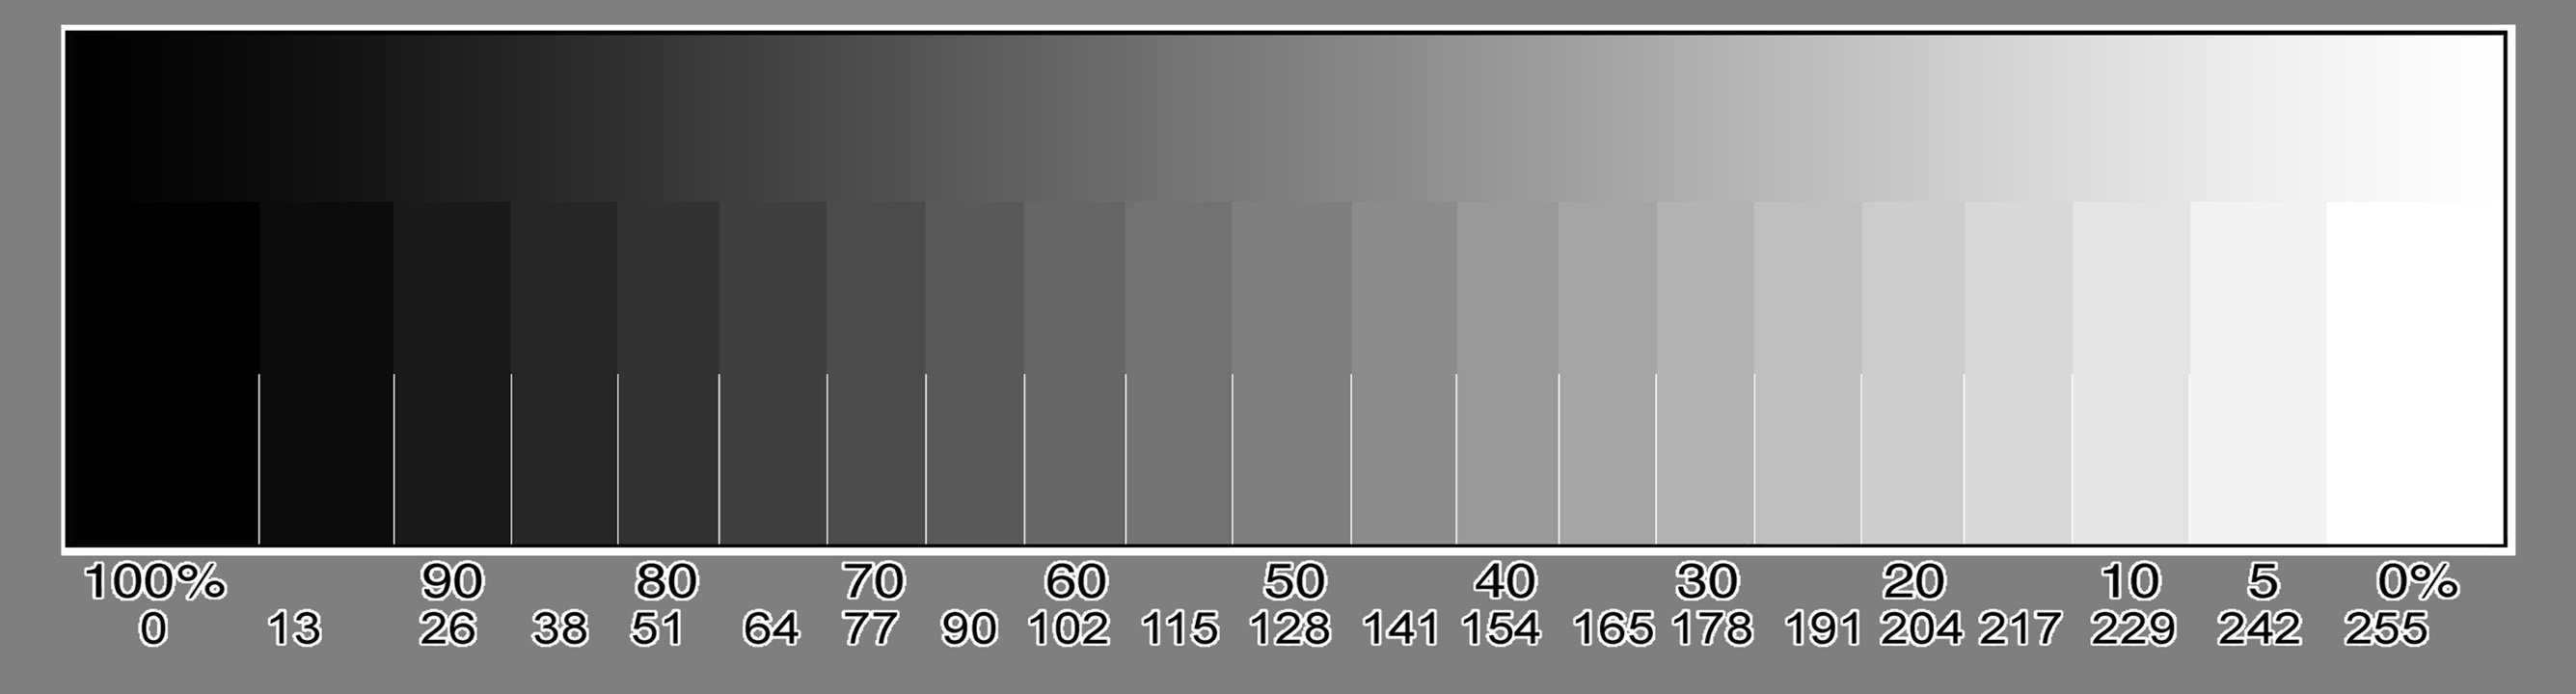
\includegraphics[width=0.5\textwidth]{figures/21stepwide8bit.jpg}  % The printed column width is 8.4 cm.
		\caption{8-bit Grayscale Shades of Gray}
		\label{fig:maxeig2}
	\end{center}
\end{figure}

Before, the data are used for training, the following preprocessing steps are used.

\subsection{Thresholding} 
Since the numbers in the dataset match the 255 shade, a simple idea for preprocessing is to use \textit{image thresholding}. 
The idea of thresholding is to compare the pixel values of the input image $f$ with some threshold $T$ and make a binary decision for the output binary image $g$ as below
\begin{align}
g(i,j) = \begin{cases}
1 & f(i,j)\ge T\\
0 & f(i,j)\le T
\end{cases}
\end{align}
for all $i, j$ where $i, j$ represent the coordinates of the $ij$\textsuperscript{th} pixel \cite{bovik2009essential}.

The output of this filter is shown in Figure \ref{fig:thresholded}

\begin{figure}
	\begin{center}
		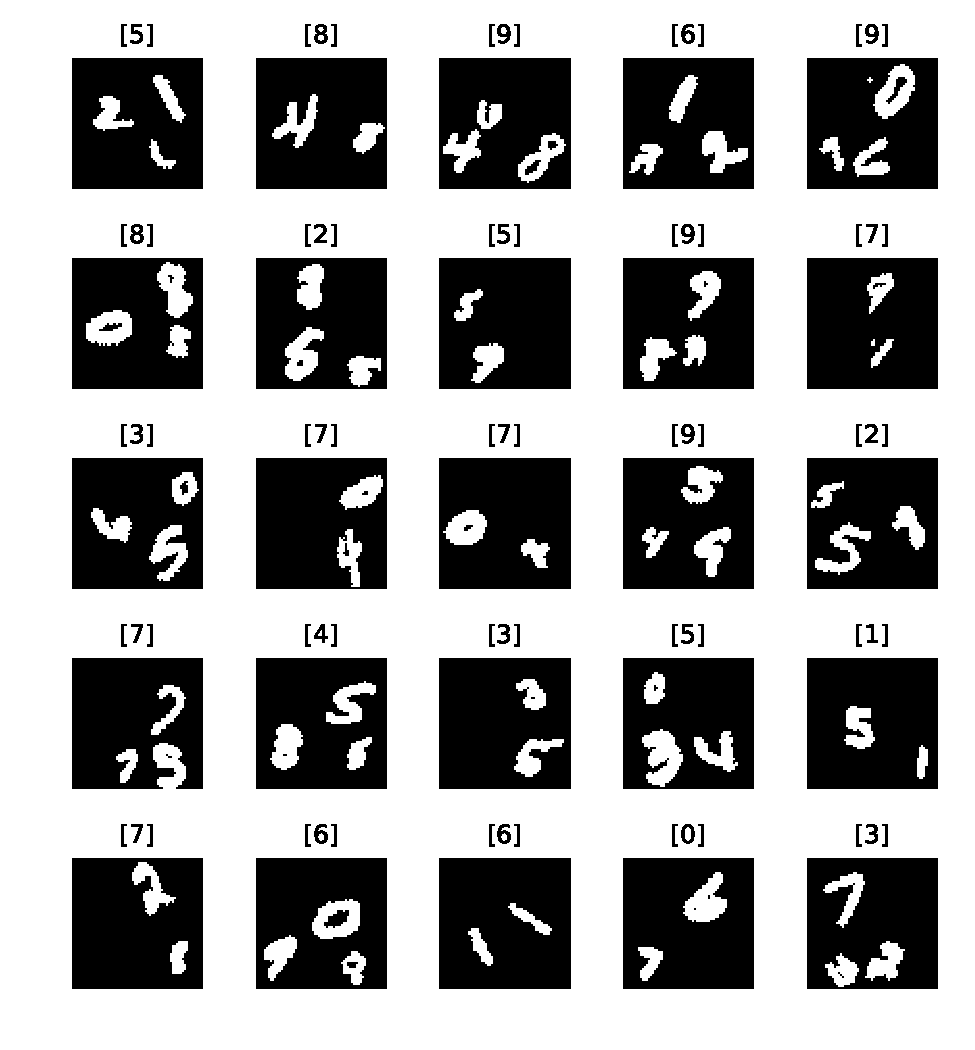
\includegraphics[width=0.4\textwidth]{figures/thresholdDataset.pdf}  % The printed column width is 8.4 cm.
		\caption{Output of thresholding on images from Figure \ref{fig:original}}
		\label{fig:thresholded}
	\end{center}
\end{figure}

\subsection{Median Filter}
The output of this filter on thresholded images are shown in Figure \ref{fig:thresholdmed}.
\begin{figure}
	\begin{center}
		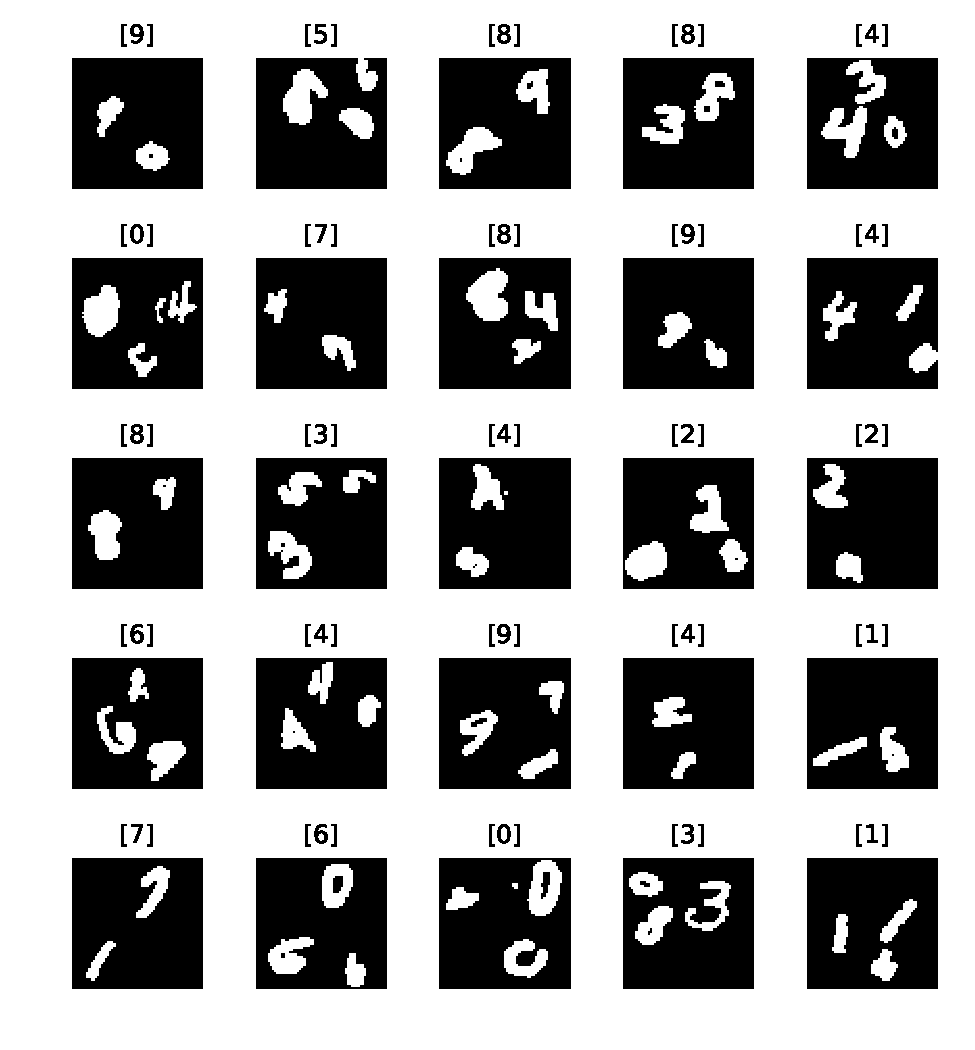
\includegraphics[width=0.4\textwidth]{figures/thresholdmedDataset.pdf}  % The printed column width is 8.4 cm.
		\caption{Output of median filter on thresholded images from Figure \ref{fig:thresholded}}
		\label{fig:thresholdmed}
	\end{center}
\end{figure}
\subsection{Biggest Number}
The output of this filter on thresholded images are shown in Figure \ref{fig:biggest}.
\begin{figure}
	\begin{center}
		\includegraphics[width=0.4\textwidth]{figures/biggestDataset.pdf}  % The printed column width is 8.4 cm.
		\caption{Output of biggest number filter on thresholded images from Figure \ref{fig:thresholded}}
		\label{fig:biggest}
	\end{center}
\end{figure}




\section{CONCLUSIONS}


\addtolength{\textheight}{-12cm}   % This command serves to balance the column lengths
                                  % on the last page of the document manually. It shortens
                                  % the textheight of the last page by a suitable amount.
                                  % This command does not take effect until the next page
                                  % so it should come on the page before the last. Make
                                  % sure that you do not shorten the textheight too much.

%%%%%%%%%%%%%%%%%%%%%%%%%%%%%%%%%%%%%%%%%%%%%%%%%%%%%%%%%%%%%%%%%%%%%%%%%%%%%%%%



%%%%%%%%%%%%%%%%%%%%%%%%%%%%%%%%%%%%%%%%%%%%%%%%%%%%%%%%%%%%%%%%%%%%%%%%%%%%%%%%



%%%%%%%%%%%%%%%%%%%%%%%%%%%%%%%%%%%%%%%%%%%%%%%%%%%%%%%%%%%%%%%%%%%%%%%%%%%%%%%%
\section*{APPENDIX}

Appendixes should appear before the acknowledgment.

\section*{STATEMENT OF CONTRIBUTIONS}
Yignan implemented the convolutional neural network.
Vincent implemented the fully-connected feedforward neural
network and the linear classifiers. Hamed implemented preprocessing and tested the linear classifiers. Yignan and Vincent implemented the algorithms on Amazon AWS. All three contributed to the report.



%%%%%%%%%%%%%%%%%%%%%%%%%%%%%%%%%%%%%%%%%%%%%%%%%%%%%%%%%%%%%%%%%%%%%%%%%%%%%%%%




\bibliographystyle{IEEEtran}
\bibliography{IEEEabrv,references}
%\begin{thebibliography}{99}
%
%\bibitem{c1} G. O. Young, �Synthetic structure of industrial plastics (Book style with paper title and editor),� 	in Plastics, 2nd ed. vol. 3, J. Peters, Ed.  New York: McGraw-Hill, 1964, pp. 15�64.
%\end{thebibliography}




\end{document}
